% This is samplepaper.tex, a sample chapter demonstrating the
% LLNCS macro package for Springer Computer Science proceedings;
% Version 2.20 of 2017/10/04
%
\documentclass[runningheads]{llncs}
%
\usepackage{graphicx}
\usepackage{amssymb}
\usepackage{amsmath}

\usepackage[ruled]{algorithm2e}
% Used for displaying a sample figure. If possible, figure files should
% be included in EPS format.
%
% If you use the hyperref package, please uncomment the following line
% to display URLs in blue roman font according to Springer's eBook style:
% \renewcommand\UrlFont{\color{blue}\rmfamily}

\begin{document}
%
\title{Bet-and-Run Strategy and MOEA/D \\ An Alternative Resource Management}
%
%\titlerunning{Abbreviated paper title}
% If the paper title is too long for the running head, you can set
% an abbreviated paper title here
%
\author{First Author\inst{1}\orcidID{0000-1111-2222-3333} \and
Second Author\inst{2,3}\orcidID{1111-2222-3333-4444} \and
Third Author\inst{3}\orcidID{2222--3333-4444-5555}}
%
\authorrunning{F. Author et al.}
% First names are abbreviated in the running head.
% If there are more than two authors, 'et al.' is used.
%
\institute{Princeton University, Princeton NJ 08544, USA \and
Springer Heidelberg, Tiergartenstr. 17, 69121 Heidelberg, Germany
\email{lncs@springer.com}\\
\url{http://www.springer.com/gp/computer-science/lncs} \and
ABC Institute, Rupert-Karls-University Heidelberg, Heidelberg, Germany\\
\email{\{abc,lncs\}@uni-heidelberg.de}}
%
\maketitle              % typeset the header of the contribution
%
\begin{abstract}
Bet-and-run strategies have been shown, both experimentally and theoretically, to be beneficial on single objective problems. Given this success and the fact that they do not take any problem knowledge into account and are not tailored to the optimization algorithms, we propose to integrate a bet-and-run strategy into the Multiobjective Evolutionary Algorithm based on Decomposition framework, (MOEA/D). 

MOEA/D represent a class of population-based metaheuristics for the solution of multicriteria optimizarion problems. It decomposes a multiobjective optimization problem into a set of scalar objective subproblems and solve this set in a collaborative way. 

\end{abstract}
%
%
%
%%%%%%%%%%%%%%%%%%%%%%%%%%%%%%%%%%%%%%%%%%%%%%%%%%%%%%%%%%%%%%%%%%
\section{Introduction}

A Multi-objective Optimization Problem (MOP)  is box-constrained problems that have $m$ multiple objective functions that must be optimized simultaneously:

\begin{align}\label{min_problem}
min f(x) = (f_1(x), f_2(x), ..., f_{n_f}(x)), \text{ subject to $x$ in $\Omega$},
\end{align}

where ${n_f}$ is the number of objective functions, $x \in \mathbb{R}^{n_v}$, the decision vector, represents a candidate solution with ${n_v}$ variables, $f: \mathbb{R}^{n_v} \rightarrow \mathbb{R}^{n_v}$ is a vector of objective functions and $\Omega$ is the feasible decision space. $\Omega$ is defined as:

\begin{align}
	\Omega =\{x \text{ in } \mathbb{R}^{n_v} | g_i(x) \leq 0 \text{ } \forall_i \text{ and } h_i(x) = 0 \text{ } \forall_j \},
\end{align}

Objectives often conflict with each other therefore no point in $\Omega$ minimizes all the objectives at the same time. Consequently, the goal of MOP solvers is to find the best trade-off that balances the different objectives in an optimal way.


Given two feasible solutions $u, v$ in $\Omega$, $u$  Pareto-dominates $v$, denoted by $f(u) \prec f(v)$, if and only if $f_k(u) \leq f_k(v), \forall_k \in \{1,..., n_f\}$ and $ f(u) \neq f(x)$. A solution $x^* \in \Omega$ is considered Pareto-Optimal if there exists no other solution $y \in \Omega$ such that $f(y) \succ f(x^*)$, i.e., if $x^*$ is non-dominated in the feasible decision space. A point is called non-dominated if no other point dominates it. That is, no single solution provides a better trade-off in all objectives.

The set of all Pareto-optimal solutions is known as the Pareto-Optimal set (PS), while the image of this set is referred to as the Pareto-optimal front (PF).\\

\begin{equation}
	PS = {x^* \in \Omega | \nexists y \in \Omega : f(y) \succ f(x^*)  },
\end{equation}

\begin{equation}
	PF = {f(x^*) | x^* \in PS }.
\end{equation}


Multi-objective evolutionary algorithms (MOEAs) have been accepted as a basic tool for approximating the PF of a MOP in a single run~\cite{zhou2011multiobjective}.Over the last two decades, many different search techniques were proposed for improving the effectiveness of multi-objective algorithms. Among them, three are the major paradigms: Pareto domination-based approaches~\cite{deb2002fast},~\cite{zitzler2001spea2}, the indicator-based approaches~\cite{beume2007sms},~\cite{zitzler2004indicator}, and the decomposition-based approaches~\cite{li2009multiobjective},~\cite{zhang2007moea}. 

MOEA/D~\cite{zhang2007moea} represents a class of population-based meta-heuristics for solving Multi Objective Problems~\cite{trivedi2017survey}. In this search paradigm, the original multi-objective problem is decomposed into simpler, single-objective sub-problems by means of scalarizations.
 However, it may waste functions evaluations searching in directions that do not present Pareto-optimal solutions~\cite{bezerra2015comparing}. 
 
 To reduce this computational cost, the allocation of resources may be better distributed among different sub-problems according to their difficulties. One way to address this problem is to adjust the behavior of the algorithm in an on-line manner to suit the problem in question~\cite{hinterding1997adaptation},~\cite{de2007parameter},~\cite{meyer2007self},~\cite{zhang2009performance},~\cite{kramer2010evolutionary},~\cite{zhang2012survey}. All algorithmic components can be tunned adaptively and often feedback information is needed for these adaptation strategies. One variation that aimed to improve this drawback is to use a dynamic/generalized resource allocation (D/G-RA) strategy which allocates resources given the difficulties of the sub-problems studied in MOEA/D-DRA by Zhang~\cite{zhang2009performance}  and  in MOEA/D-GRA Zhou et. al~\cite{zhou2016all}.
 
Another approach that could help reducing the amount of functions evaluations is to use restart strategies. That might help if the algorithm is wasting evaluations searching in directions that are not promising, the algorithm is restarted and a new initial set of solutions is sampled. It is well known that the initial set of solutions often influences the quality outcome, but by simpling re-sample the set of solutions might not direct the algorithm to a more promising region of the search space. Therefore one more elaborated strategy that considers different initial set of solutions may positively address the final quality of the results.
 
One strategy that consideres different initial set of solutions is the Bet-and-Run strategy~\cite{fischetti2014exploiting}. It extends two typical uses for an algorithm with budget \textit{t} are to use all of the budget for a single run of the algorithm or to make a number of \textit{k} runs of the algorithm and run each with \textit{t/k}. In this strategy, \textit{k} independent runs are all executed with a fraction of the total budget and the best among them continues with the remaining of the total budget.
 
From a theoretical point of view, the way that this strategy relates with initialization can be beneficial even on easy functions and be an effective countermeasure against problems with promising but deceptive regions. However, this benefit come with a cost which is the introduction of two additional control parameters, that are non-trivial to be chosen~\cite{lissovoi2017theoretical}.

The main contributions of this paper can be summarized as follows:

\begin{itemize}
	\item A careful examination of the proper settings of the hyper-parameters of the Bet-and-Run strategy when combined with the two variants (MOEA/D~\cite{zhang2007moea} and MOEA/D-DE~\cite{li2009multiobjective}) of MOEA/D with Bet-and-Run strategy which realize the best performance of the MOEAs on the 10 CEC2009 competition functions~\cite{zhang2008multiobjective}.
	\item Proposition an alternative way of choosing the MOEA/D variants hyper-parameters by randomly selecting them.		
	\item An extensive analysis of the performance of using the hyper-volume indicator~\cite{zitzler1998multiobjective}, the epsilon indicator~\cite{zitzler2003performance}, and the IGD indicator~\cite{zitzler2003performance} on the 7-DTLZ~\cite{deb2005scalable} and the 9-WFG~\cite{huband2006review}. 
\end{itemize}


 
 

\section{MOEA/D}\label{sec:background} 

\begin{figure*}[!t]\label{decomp-example}
	\centering
	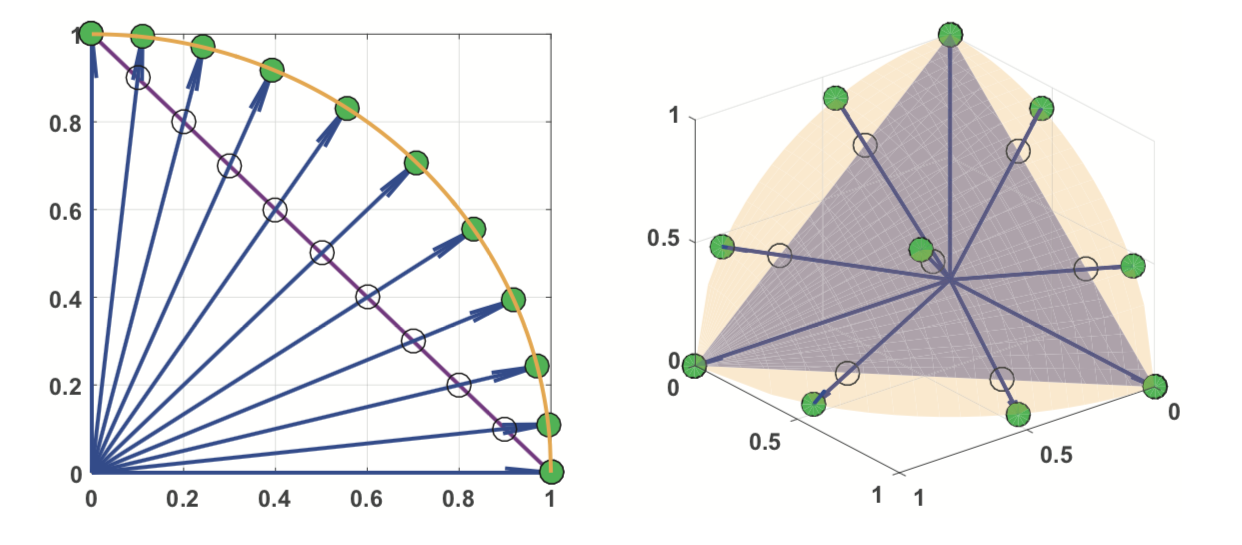
\includegraphics[width=\textwidth]{images/decomp2.png}
	\caption{Decomposition  -  2 and 3 objectives - Figure from \cite{chugh2017handling} }
\end{figure*}.

Here, MOEA/D~\cite{zhang2007moea} is briefly explained. MOEA/D represents a class of population-based meta-heuristics for solving Multi Objective Problems (MOPs). It is based on decomposition, which is one kind of scalarizing function, where one multi-objective problem becomes various single-objective sub-problem. That is, MOEA/D decomposes an MOP with $n_f$ objectives, as defined in equation~\ref{min_problem}, into $N$  sub-problems using a set of uniformly distributed weight vectors. To define the sub-problem a weight vector is used as a decomposition strategy to  define the sub-problems.  All these $N$ sub-problems are expected to represent a good approximation to the PF, as it is shown in Figure~\ref{decomp-example}.

MOEA/D solves these subproblems simultaneously by evolving a set of solutions in a single run by using a aggregation function. This function allied with the weight vectors need to guarantee that a optimal solution to a sub-problem is Pareto-optimal for the MOP and also need to guarantee that the solutions are well distributed in the space of objectives. Therefore, the set of solutions may provide a fair approximation of the Pareto Front.

The relationship between the set of solutions and the sub-problems is formulated as for every sub-problem a unique solution is associated to it, thus the size of the set of solutions is equal to the number of sub-problems.  At each interaction, one new candidate solution is generated by applying a sequence of variation operators to the existing solutions. This new solution is then compared with the old one, and the best solution after is maintained as the incumbent solution given the procedure defined by the update strategy.

To compare the solutions or to generate a new one, the algorithm utilizes a neighborhood that defines the limits the exchange of information of a sub-problem between candidates solutions. This neighborhood is defined based on the distance among their weights.



\IncMargin{1em}
\begin{algorithm}
\LinesNumbered
	\KwIn{Objective functions \textbf{f}; constraint functions \textbf{g}; input parameters}
	t$\rightarrow$ 0\\
	\textit{run} $\rightarrow$ TRUE\\
	Initialize the solution set $ X^{(t)} =  {x^1, ..., x^{n_{f}}}$ by random sampling from $\Omega$
	Generate weights $\Lambda$\\
	%
	%\For{$i \in {1,...,n_f}$}{Set the neighborhood index list $B^i = {1_i, ..., i_T}$;}
	%
	%
	\While{run}{
		Define or update neighborhood $B^i = {1_i, ..., i_{n_{f}} } $\\
		Copy incumbent solution set $X'^{(t)}$ into $X'^{(t)} $\\
		\For{each variation operator $v \in V$}{
			$X^{(t)} \leftarrow v(X'^{(t)})$
		}
	Evaluate solutions in $X^{(t)}$ and $X'^{(t)} $
	
	Define next population $X^{(t+1)}$
	Update \textit{run}  flag
	t$\rightarrow$ t + 1
	}
	\textbf{return} 	$X^{(t)}$, f$(X^{(t)})$
	%		
	%		
	\caption{General procedure of MOEA/D framework}
\end{algorithm}\DecMargin{1em}


 
%%%%%%%%%%%%%%%%%%%%%%%%%%%%%%%%%%%%%%%%%%%%%%%%%%%%%%%%%%%%%%%%%%
\section{Bet-and-Run}\label{intro}

\subsection{Restart Strategy}
Restart Strategies are a mechanism helps the algorithm to explore more in the solution area~\cite{yu2018simulated}. For instance, stochastic algorithms and randomized search heuristics may encounter some stagnation before finding a high quality solution. One way to overcome  such stagnation is to introduce a restart strategy, since it forcibly changes the search points by restoring the algorithm to its beginning~\cite{kanahara2018restart}. Also, Restart Strategy might be used to avoid heavy-tailed running time distributions \cite{gomes2000heavy}, because if a execution of an algorithm does not conclude within a pre determined limit or if the solution quality is unsatisfactory, the algorithm is restarted~\cite{lissovoi2017theoretical}. Finally, it may be considered as an additional speed-up \cite{friedrich2017generic}.

\subsection{Bet-and-Run framework}


Fischetti and Monaci~\cite{fischetti2014exploiting} investigated the Bet-and-Run framework. They defined it as a number of short runs with randomized initial conditions (the bet-phase) and then bet on the most promising run(the bet-phase) and bring it to completion. In their work, they studied the following Bet-and-Run framework:\\


\indent \textbf{Phase 1} performs \textit{k} runs of the algorithm for some short time limit \textit{$t_1$} with $t_1 \leq t/k$.\\
\indent \textbf{Phase 2} uses remaining time $t_2 = t - k*t_1$ to continue \textit{only the best run} from the first phase until time out. \\

In 2017, Lissovoi and Sudholt~\cite{lissovoi2017theoretical} analyzed this framework theoretically. They investigate it in the context of single objective problems and found that new initializations can have a small beneficial effect even on very easy functions, that this restart strategy might be an effective countermeasure when problems with promising and deceptive regions are encountered.


To the best of our knowledge, the Bet-and-Run framework was only applied with evolutionary algorithms in the context of single objective problems. 

% arrumar o where...
\section{MOEA/D and Bet-and-Run}

In this work, we propose to integrate both frameworks, the MOEA/D the Bet-and-Run.  First, the implementation of MOEA/D is discussed. Then the implementation of the Bet-and-Run followed by the discussion of how to integratate them.

\subsection{MOEA/D}

In this paper, two different MOEA/D combinations found in the literature  were studied. These combinations are the original MOEA/D~\cite{zhang2007moea} and MOEA/D-DE~\cite{li2009multiobjective}. 

The first modification was to change the parameter control $H$ of the simplex-lattice design (SLD) that is used to generate the weight vectors W. For the 2-objective problem benchmark functions it was set as \textit{199}, while for the 3-objective problem benchmark functions, \textit{19}. Those vales for the $H$ parameter were chosen so that the number of sub-problems and the size of incumbent solutions are equal to \textit{200}, following default settings as in the recent work from Tanabe et. al~\cite{tanabe2018analysis}. Na verdade eles usam varios tamanhos de populacao, e percebem que menor e melhor no inicio e pior no fim. The other modification was to use an archive, that stores all nondominated solutions found during the search process.(????????). 

We also studied the integration of On-line Resource Allocation (ONRA), proposed in the context of MOEA/D by \cite{zhou2016all}. The resource distribution when using ONRA is allocated using an adaptative strategy aiming to adjust the behaviour of an algorithm in on-line manner to suit the problem in question. Although, other strategies were proposed in the work of Zhou, ONRA was the one that perfomed better among all strategies proposed. The ONRA strategy is concerned with the distribution of resources in an execution of MOEA/D. Different amounts of resources are considered to different sub-problems, following the assumption that some sub-problems can be more difficult to approximate that others. 

\subsection{Bet-and-Run}

In this work, the Bet-and-run framework implemented follows the results found  by Friedrich et. al~\cite{friedrich2017generic}. They studied different combinations strategies that are diverse on the amount of resources assigned for phase 1 and 2. 

The best overall strategy found is the one that uses 40\% of the total budget available on short runs (phase1) and then run the most prominient one (phase 2) with the remaining 60\% of the budget found. One adjusment was made to better fit the context of MOP and MOEA/D which is defining the budget as the number of interactions, instead of using time as the budget as Friedrich et. al used.

%Phase 1 of the bet-and-run strategy is using the epsilon indicator. 40 instances.
%It needs two Pareto sets. The first is the Pareto set of a bet instance while the other is the Pareto set from the control algorithm executed with 1% of the number of interactions. 
%Phase 2 uses the 60% rest of max interactions.


%
\section{Experiment Design}

The DTLZ~\cite{deb2005scalable} and the ZDT~\cite{zitzler2000comparison},test problems were used in the analysis. For the first the number of objectives used was two three. According to~\cite{deb2005scalable}, for the DTLZ problems, the number of position variables D was set to $k = 5$ for the DTLZ1 problem, $k = 7$ for the DTLZ2 problem and $k = 10$ for the other DTLZ problems, where the number of variables $D = n_f + k -1$. For the ZDT the number of variable $D = 11$.

Our limit budget was set to the maximum of iteractions, with value of 300, which leads to a number of functions evaluations of XXXXX.


The hypervolume (HV) indicator~\cite{zitzler1998multiobjective} was used. ishibuchi2018specify
Compared with their HV - normalized between 0 and 1 (based on the fair comparison paper).
30 repetitions.
box-plots 
Kruskal-Wallis (data non-normal data, used in the literature)

Configurations and Parameters

Control - Based on the common variation: MOEA/D (variation1) and MOEA/D-DE as in preset\_moead
Control and ONRA - parameters: dt = 20
Ben-and-run
Ben-and-run and ONRA - parameters: dt = 20

Dt - interval that control the resources allocation. From the proposal paper, there is no much sensibility.
Decomposition method used - SLD, with H being 199 for 2D and 19 for 3D 
number of dimensions - 60 
All other parameters are defined by  preset\_moead

Bet-and-run

Phase 1 of the bet-and-run strategy is using the epsilon indicator. 40 instances.
It needs two Pareto sets. The first is the Pareto set of a bet instance while the other is the Pareto set from the control algorithm executed with 1\% of the number of interactions. 
Phase 2 uses the 60\% rest of max interactions.

\section{Evaluation Metrics}

Evaluation Metrics

Unary Indicators

- Measure Pareto Sets independently.
- Power is restricted.
- Cannot tell in general if a set is better than another.
- Focus on problem dependent and specifics.
- Assumptions and knowledge should be specified.
1. Hyper-volume.
2. Error ratio.
3. Distance from reference set.

Binary Indicators

- Theoretically have no limitations.
- Analysis and presentation of results more difficult.

1. R1, R2, R3 indicators.
2. $\varepsilon$-Indicator.
3. Binary Hyper-volume.

Hypervolume
Considerations

- Is complete - If, and only if $HV(A) > HV(B) \implies A$ is not worse than $B$.
- Is weakly compatible - $HV(A) > HV(B) \implies \not B$ dominates $A$.
- Assumptions - All points of a Pareto Set under consideration dominate the reference point.
- @ishibuchi2018specify proposed a method to specify the reference point from a viewpoint of fair performance comparison.

Considerations
- A large population size is **always** more beneficial than a small one.
- Measures both the convergence toward the Pareto Front and the diversity of non-dominated solutions.
- A monotonic increase of the hyper-volume over time cannot always be ensured.
- For MOEA/D that is always true.

$\varepsilon$-Indicator
Considerations
- It compares 2 Pareto Sets.
- It indicates which set is better and how much better
- If A is better than B $\implies I_{\varepsilon}(B,A) > 0$.
- If $I_{\varepsilon}(A,B) \leq 0$ and $I_{\varepsilon}(B,A) > 0 \implies A$ is better than $B$.

The benchmark used are the DTLZ and the ZDT group of functions.

DTLZ are easy~\cite{bezerra2015comparing}.


\section{Results}\label{sec:results}


Analysis are done with 

\section{Conclusion}
\label{sec:conclusion}



\bibliographystyle{splncs04}
\bibliography{bib} 



\end{document}
